% =========================================================================
% BÀI 26: ĐƠN VỊ ĐO ĐỘ DÀI (CHỦ ĐỀ 7 - ĐỘ DÀI VÀ ĐO ĐỘ DÀI - TOÁN LỚP 1)
% TOÀN BỘ CÂU HỎI ĐƯỢC VẼ HÌNH MINH HỌA TRỰC QUAN 100% BẰNG TIKZ 2D & 3D
% =========================================================================

% --- CÁC HÀM VẼ HÌNH TRỰC QUAN ĐẶC TRƯNG CHO BÀI 26 ---

% 1. Cây thước kẻ chia vạch xăng-ti-mét (cm)
\providecommand{\VeThuocChiaCm}[3][cyan]{% #1=màu thước, #2=độ dài cm tối đa, #3=(x,y)
  \begin{scope}[shift={(#3)}, scale=0.7]
    \draw[fill=#1!20, draw=black!80, line width=0.8pt, rounded corners=2pt] (-0.3,-0.5) rectangle (#2+0.5,0.5);
    \node[font=\bfseries\tiny, color=#1!80!black] at (-0.05,-0.25) {cm};
    \foreach \x in {0,1,...,#2} {
      \draw[black!85, line width=0.6pt] (\x,0.5) -- (\x,0.15);
      \node[below, font=\tiny\bfseries] at (\x,0.15) {\x};
      \ifnum\x<#2
        \draw[black!60, line width=0.4pt] (\x+0.5,0.5) -- (\x+0.5,0.3);
      \fi
    }
  \end{scope}
}

% 2. Vật đặt trên thước từ vạch 0
\providecommand{\VeVatTrenThuoc}[5]{% #1=vạch bắt đầu, #2=chiều dài, #3=màu vật, #4=(x,y), #5=tên vật
  \begin{scope}[shift={(#4)}, scale=0.7]
    \draw[fill=#3!50, draw=black!80, line width=0.7pt, rounded corners=1.5pt] (#1,0.55) rectangle (#1+#2,0.95);
    \node[font=\bfseries\tiny, color=black] at (#1+#2/2,0.75) {#5};
    \draw[line width=0.6pt, red!85, dashed] (#1,0.5) -- (#1,1.05);
    \draw[line width=0.6pt, red!85, dashed] (#1+#2,0.5) -- (#1+#2,1.05);
  \end{scope}
}

% 3. Đoạn thẳng có mút tròn và nhãn độ dài
\providecommand{\VeDoanThangCm}[5]{% #1=(x,y), #2=độ dài cm, #3=điểm đầu, #4=điểm cuối, #5=số đo
  \begin{scope}[shift={(#1)}, scale=0.65]
    \draw[line width=2pt, blue!85] (0,0) -- (#2,0);
    \fill[red!80] (0,0) circle (0.12cm) node[above=2pt, font=\bfseries\scriptsize, color=black] {#3};
    \fill[red!80] (#2,0) circle (0.12cm) node[above=2pt, font=\bfseries\scriptsize, color=black] {#4};
    \draw[line width=0.8pt, stealth-stealth, orange!90!black] (0,-0.4) -- (#2,-0.4) node[midway, below, font=\bfseries\scriptsize] {#5};
  \end{scope}
}

% =========================================================================
% BẮT ĐẦU NỘI DUNG 20 CÂU HỎI
% =========================================================================

\textbf{Phần 1. Trắc nghiệm lựa chọn}
\setcounterpageref{ex}{0}

% --- TRANG 1: CÂU 1 ĐẾN CÂU 4 ---

% CÂU 1: Kí hiệu của xăng-ti-mét
\begin{ex} %[1H7N26]
Quan sát kí hiệu đơn vị đo độ dài trên đầu cây thước kẻ:
\begin{center}\vspace{-2.5mm}
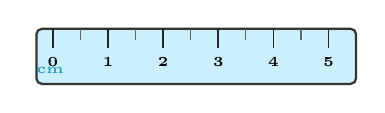
\begin{tikzpicture}
  \VeThuocChiaCm[cyan]{5}{0,0}
\end{tikzpicture}
\vspace{-2.5mm}\end{center}
Đơn vị xăng-ti-mét được viết tắt là:
\begin{multicols}{4}
\choice
{$\text{m}$}
{$\text{kg}$}
{$\text{l}$}
{\True $\text{cm}$}
\end{multicols}
\loigiai{
Xăng-ti-mét viết tắt là $\text{cm}$.\\
\textbf{Đáp án: D.}
}
\end{ex}

% CÂU 2: Dụng cụ và đơn vị đo đoạn thẳng
\begin{ex} %[1H7N26]
Cục tẩy được đặt vừa khít từ vạch $0$ đến vạch $4$ trên thước:
\begin{center}\vspace{-2.5mm}
\begin{tikzpicture}
  \VeThuocChiaCm[cyan]{6}{0,0}
  \VeVatTrenThuoc{0}{4}{pink}{0,0}{Cục tẩy}
\end{tikzpicture}
\vspace{-2.5mm}\end{center}
Cục tẩy dài $4\text{ cm}$. Để đo độ dài vật ngắn, ta dùng thước chia theo đơn vị:
\begin{multicols}{2}
\choice
{Ki-lô-gam}
{\True Xăng-ti-mét}
{Lít}
{Giờ}
\end{multicols}
\loigiai{
Để đo độ dài các vật ngắn, người ta dùng thước có vạch chia xăng-ti-mét ($\text{cm}$).\\
\textbf{Đáp án: B.}
}
\end{ex}

% CÂU 3: Phép cộng hai độ dài 5 cm + 3 cm
\begin{ex} %[1H7H26]
Ghép đoạn thẳng $5\text{ cm}$ nối tiếp với đoạn thẳng $3\text{ cm}$:
\begin{center}\vspace{-2.5mm}
\begin{tikzpicture}[scale=0.6]
  \draw[line width=2.5pt, blue!80] (0,0) -- (3.5,0);
  \draw[line width=2.5pt, orange!90] (3.5,0) -- (5.6,0);
  \node[above, font=\bfseries\tiny, color=blue!90!black] at (1.75,0.1) {$5\text{ cm}$};
  \node[above, font=\bfseries\tiny, color=orange!90!black] at (4.55,0.1) {$3\text{ cm}$};
  \draw[line width=0.8pt, stealth-stealth, red!85] (0,-0.35) -- (5.6,-0.35) node[midway, below, font=\bfseries\tiny] {Cả hai đoạn: ?};
\end{tikzpicture}
\vspace{-2.5mm}\end{center}
Tính: $5\text{ cm} + 3\text{ cm} = \dots$
\begin{multicols}{4}
\choice
{$7\text{ cm}$}
{$9\text{ cm}$}
{$10\text{ cm}$}
{\True $8\text{ cm}$}
\end{multicols}
\loigiai{
Ta cộng các số rồi viết thêm đơn vị đo: $5 + 3 = 8\text{ cm}$.\\
\textbf{Đáp án: D.}
}
\end{ex}

% CÂU 4: Phép trừ độ dài 9 cm - 4 cm
\begin{ex} %[1H7H26]
Băng giấy dài $9\text{ cm}$, cắt bớt đi một đoạn $4\text{ cm}$:
\begin{center}\vspace{-2.5mm}
\begin{tikzpicture}[scale=0.6]
  \draw[fill=green!40, draw=black] (0,0) rectangle (3.5,0.5) node[midway, font=\bfseries\tiny] {Còn lại ? cm};
  \draw[fill=gray!30, draw=black, dashed] (3.5,0) rectangle (6.3,0.5) node[midway, font=\bfseries\tiny] {Cắt $4\text{ cm}$};
  \draw[line width=0.8pt, stealth-stealth, blue!85] (0,-0.3) -- (6.3,-0.3) node[midway, below, font=\bfseries\tiny] {Ban đầu $9\text{ cm}$};
\end{tikzpicture}
\vspace{-2.5mm}\end{center}
Tính: $9\text{ cm} - 4\text{ cm} = \dots$
\begin{multicols}{4}
\choice
{\True $5\text{ cm}$}
{$4\text{ cm}$}
{$6\text{ cm}$}
{$7\text{ cm}$}
\end{multicols}
\loigiai{
$9 - 4 = 5\text{ cm}$.\\
\textbf{Đáp án: A.}
}
\end{ex}

\newpage
% --- TRANG 2: CÂU 5 ĐẾN CÂU 8 ---

% CÂU 5: Cộng số tròn chục kèm cm
\begin{ex} %[1H7H26]
Hai thanh gỗ tròn chục được ghép lại:
\begin{center}
\begin{tikzpicture}[scale=0.65]
  \draw[fill=cyan!35, draw=black!80, line width=0.6pt] (0,0) rectangle (2.0,0.6) node[midway, font=\bfseries\scriptsize] {$10\text{ cm}$};
  \draw[fill=yellow!45, draw=black!80, line width=0.6pt] (2.0,0) rectangle (6.0,0.6) node[midway, font=\bfseries\scriptsize] {$20\text{ cm}$};
  \draw[line width=1pt, stealth-stealth, red!85] (0,-0.35) -- (6.0,-0.35) node[midway, below, font=\bfseries\scriptsize] {Tổng chiều dài = ?};
\end{tikzpicture}
\end{center}
Tính: $10\text{ cm} + 20\text{ cm} = \dots$
\begin{multicols}{4}
\choice
{$25\text{ cm}$}
{$35\text{ cm}$}
{\True $30\text{ cm}$}
{$40\text{ cm}$}
\end{multicols}
\loigiai{
$10\text{ cm} + 20\text{ cm} = 30\text{ cm}$.\\
\textbf{Đáp án: C.}
}
\end{ex}

% CÂU 6: Trừ số tròn chục kèm cm
\begin{ex} %[1H7H26]
Thanh nhôm dài $50\text{ cm}$, cắt đi một đoạn $20\text{ cm}$:
\begin{center}
\begin{tikzpicture}[scale=0.65]
  \draw[fill=teal!30, draw=black!80, line width=0.6pt] (0,0) rectangle (3.6,0.6) node[midway, font=\bfseries\scriptsize] {Còn lại ? cm};
  \draw[fill=gray!30, draw=black, dashed] (3.6,0) rectangle (6.0,0.6) node[midway, font=\bfseries\scriptsize] {$20\text{ cm}$};
  \draw[line width=1pt, stealth-stealth, blue!85] (0,-0.35) -- (6.0,-0.35) node[midway, below, font=\bfseries\scriptsize] {Ban đầu $50\text{ cm}$};
\end{tikzpicture}
\end{center}
Tính: $50\text{ cm} - 20\text{ cm} = \dots$
\begin{multicols}{4}
\choice
{$25\text{ cm}$}
{\True $30\text{ cm}$}
{$35\text{ cm}$}
{$40\text{ cm}$}
\end{multicols}
\loigiai{
$50\text{ cm} - 20\text{ cm} = 30\text{ cm}$.\\
\textbf{Đáp án: B.}
}
\end{ex}

% CÂU 7: Tính độ dài đường gấp khúc gồm 2 đoạn AB và BC
\begin{ex} %[1H7V26]
Đoạn thẳng $AB$ dài $8\text{ cm}$, đoạn thẳng $BC$ dài $6\text{ cm}$:
\begin{center}
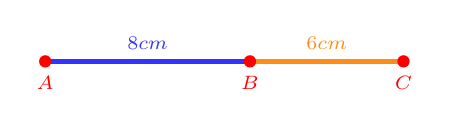
\begin{tikzpicture}[scale=0.65]
  \draw[line width=2pt, blue!80] (0,0) -- (4,0) node[midway, above, font=\bfseries\scriptsize] {$8\text{ cm}$};
  \draw[line width=2pt, orange!90] (4,0) -- (7,0) node[midway, above, font=\bfseries\scriptsize] {$6\text{ cm}$};
  \fill[red] (0,0) circle (0.12cm) node[below=2pt, font=\bfseries\scriptsize] {$A$};
  \fill[red] (4,0) circle (0.12cm) node[below=2pt, font=\bfseries\scriptsize] {$B$};
  \fill[red] (7,0) circle (0.12cm) node[below=2pt, font=\bfseries\scriptsize] {$C$};
\end{tikzpicture}
\end{center}
Cả hai đoạn thẳng dài tất cả là:
\begin{multicols}{4}
\choice
{\True $14\text{ cm}$}
{$13\text{ cm}$}
{$15\text{ cm}$}
{$16\text{ cm}$}
\end{multicols}
\loigiai{
Cả hai đoạn thẳng dài tất cả là: $8 + 6 = 14\text{ cm}$.\\
\textbf{Đáp án: A.}
}
\end{ex}

% CÂU 8: Sợi dây bị cắt bớt
\begin{ex} %[1H7V26]
Sợi dây len dài $18\text{ cm}$, bạn Mai cắt bớt đi $5\text{ cm}$:
\begin{center}
\begin{tikzpicture}[scale=0.65]
  \draw[line width=2.5pt, purple!70] (0,0) -- (4.2,0);
  \node[above, font=\bfseries\tiny, color=purple!90!black] at (2.1,0.1) {Còn lại ? cm};
  \draw[line width=2pt, gray!60, dashed] (4.2,0) -- (6.0,0);
  \node[above, font=\bfseries\tiny, color=gray!80!black] at (5.1,0.1) {Bắt $5\text{ cm}$};
  \draw[line width=0.8pt, stealth-stealth, blue!80] (0,-0.4) -- (6.0,-0.4) node[midway, below, font=\bfseries\tiny] {Cả sợi dây: $18\text{ cm}$};
\end{tikzpicture}
\end{center}
Sợi dây len còn lại dài là:
\begin{multicols}{4}
\choice
{$12\text{ cm}$}
{$14\text{ cm}$}
{\True $13\text{ cm}$}
{$15\text{ cm}$}
\end{multicols}
\loigiai{
Sợi dây còn lại dài: $18 - 5 = 13\text{ cm}$.\\
\textbf{Đáp án: C.}
}
\end{ex}

\newpage
% --- TRANG 3: CÂU 9 ĐẾN CÂU 12 ---

% CÂU 9: So sánh biểu thức với số đo
\begin{ex} %[1H7V26]
Cân đĩa so sánh hai vế: bên trái là $12\text{ cm} + 5\text{ cm}$, bên phải là $18\text{ cm}$:
\begin{center}

\begin{tikzpicture}[scale=0.65]
  \node[draw=blue!80, fill=cyan!15, rounded corners=3pt, font=\bfseries\normalsize, inner sep=4pt] at (-2.2,0) {$12\text{ cm} + 5\text{ cm}$};
  \node[draw=orange!90, fill=yellow!30, rounded corners=2pt, font=\bfseries\normalsize, inner sep=3pt] at (0.2,0) {~?~};
  \node[draw=red!80, fill=pink!20, rounded corners=3pt, font=\bfseries\normalsize, inner sep=4pt] at (2.2,0) {$18\text{ cm}$};
\end{tikzpicture}
\end{center}
Dấu thích hợp để điền vào ô trống là:
\begin{multicols}{4}
\choice
{\True $<$}
{$>$}
{$=$}
{$+$}
\end{multicols}
\loigiai{
Tính vế trái: $12\text{ cm} + 5\text{ cm} = 17\text{ cm}$.\\
Vì $17\text{ cm} < 18\text{ cm}$ nên dấu cần điền là $<$.\\
\textbf{Đáp án: A.}
}
\end{ex}

% CÂU 10: Biểu thức có hai phép tính
\begin{ex} %[1H7V26]
Ba đoạn thước được cộng trừ liên tiếp:
\begin{center}

\begin{tikzpicture}[scale=0.7]
  \node[draw=blue!80, fill=cyan!10, rounded corners=3pt, font=\bfseries\normalsize, inner sep=4pt] at (0,0) {
    $15\text{ cm} - 5\text{ cm} + 8\text{ cm} = \dots$
  };
\end{tikzpicture}
\end{center}
Giá trị của biểu thức trên là:
\begin{multicols}{4}
\choice
{$16\text{ cm}$}
{$20\text{ cm}$}
{$17\text{ cm}$}
{\True $18\text{ cm}$}
\end{multicols}
\loigiai{
Thực hiện từ trái sang phải: $15 - 5 = 10\text{ cm}$; sau đó $10 + 8 = 18\text{ cm}$.\\
\textbf{Đáp án: D.}
}
\end{ex}

% CÂU 11: Bút chì và cục tẩy
\begin{ex} %[1H7V26]
Đo bút chì và cục tẩy:
\begin{center}
\begin{tikzpicture}[scale=0.65]
  \draw[fill=yellow!50, draw=black] (0,0.3) rectangle (4.9,0.7) node[midway, font=\tiny\bfseries] {Bút chì: $14\text{ cm}$};
  \draw[fill=cyan!40, draw=black] (0,-0.4) rectangle (1.4,0) node[midway, font=\tiny\bfseries] {Tẩy: $4\text{ cm}$};
  \draw[line width=1pt, stealth-stealth, red!85] (1.4,-0.2) -- (4.9,-0.2) node[midway, below, font=\bfseries\tiny] {Dài hơn ? cm};
\end{tikzpicture}
\end{center}
Bút chì dài hơn chiếc tẩy bao nhiêu xăng-ti-mét?
\begin{multicols}{4}
\choice
{$9\text{ cm}$}
{$11\text{ cm}$}
{\True $10\text{ cm}$}
{$12\text{ cm}$}
\end{multicols}
\loigiai{
Bút chì dài hơn cục tẩy số xăng-ti-mét là: $14 - 4 = 10\text{ cm}$.\\
\textbf{Đáp án: C.}
}
\end{ex}

% CÂU 12: Vận dụng cao - Dán chồng hai băng giấy
\begin{ex} %[1H7C26]
Dán nối băng giấy xanh ($20\text{ cm}$) và đỏ ($30\text{ cm}$) chồng lên nhau $2\text{ cm}$:
\begin{center}
\begin{tikzpicture}[scale=0.6]
  \draw[fill=cyan!40, draw=black] (0,0) rectangle (3.0,0.6) node[midway, font=\tiny\bfseries] {Xanh $20\text{ cm}$};
  \draw[fill=red!40, draw=black] (2.7,0) rectangle (7.0,0.6) node[midway, font=\tiny\bfseries] {Đỏ $30\text{ cm}$};
  \draw[fill=purple!60, draw=black] (2.7,0) rectangle (3.0,0.6);
  \node[above, font=\bfseries\tiny, color=purple!90!black] at (2.85,0.65) {Chồng $2\text{ cm}$};
\end{tikzpicture}
\end{center}
Chiều dài của băng giấy mới sau khi dán là:
\begin{multicols}{4}
\choice
{$50\text{ cm}$}
{\True $48\text{ cm}$}
{$46\text{ cm}$}
{$52\text{ cm}$}
\end{multicols}
\loigiai{
Tổng hai băng giấy là $20 + 30 = 50\text{ cm}$. Do dán chồng lên nhau $2\text{ cm}$ nên chiều dài mới là: $50 - 2 = 48\text{ cm}$.\\
\textbf{Đáp án: B.}
}
\end{ex}

\newpage
% --- TRANG 4: CÂU 13 ĐẾN CÂU 16 (ĐÚNG / SAI) ---

\textbf{Phần 2. Trắc nghiệm đúng sai}
\setcounterpageref{ex}{0}

% CÂU 13: Quy tắc tính toán có đơn vị đo cm
\begin{ex} %[1H7H26]
Các phép tính độ dài trên bảng lớp:
\begin{center}
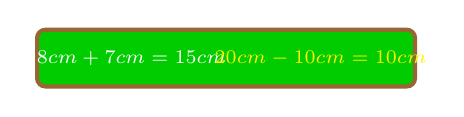
\begin{tikzpicture}[scale=0.6]
  \draw[fill=green!80!black, draw=brown!80!black, line width=1.5pt, rounded corners=3pt] (-4,-0.6) rectangle (4,0.6);
  \node[font=\bfseries\scriptsize, color=white] at (-2,0) {$8\text{ cm} + 7\text{ cm} = 15\text{ cm}$};
  \node[font=\bfseries\scriptsize, color=yellow] at (2,0) {$20\text{ cm} - 10\text{ cm} = 10\text{ cm}$};
\end{tikzpicture}
\end{center}
Xét tính đúng hoặc sai của các khẳng định sau:
\choiceTF
{\True Phép tính $8\text{ cm} + 7\text{ cm} = 15\text{ cm}$ là đúng.}
{\True Phép tính $20\text{ cm} - 10\text{ cm} = 10\text{ cm}$ là đúng.}
{Viết kết quả $15\text{ cm} - 5\text{ cm} = 10$ là đầy đủ và chính xác.}
{\True Kết quả của phép tính có đơn vị đo bắt buộc phải ghi kèm tên đơn vị $\text{cm}$.}
\loigiai{
\begin{itemize}
  \item a) \textbf{Đúng}: $8 + 7 = 15\text{ cm}$.
  \item b) \textbf{Đúng}: $20 - 10 = 10\text{ cm}$.
  \item c) \textbf{Sai}: Thiếu tên đơn vị $\text{cm}$.
  \item d) \textbf{Đúng}: Phải viết là $10\text{ cm}$.
\end{itemize}
}
\end{ex}

% CÂU 14: Hai đoạn thẳng AB và CD
\begin{ex} %[1H7V26]
Đoạn thẳng $AB$ dài $12\text{ cm}$ và đoạn thẳng $CD$ dài $16\text{ cm}$:
\begin{center}
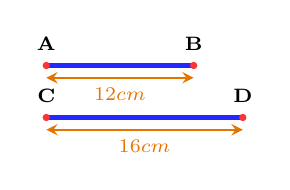
\begin{tikzpicture}[scale=0.6]
  \VeDoanThangCm{0,0.5}{4.8}{A}{B}{$12\text{ cm}$}
  \VeDoanThangCm{0,-0.6}{6.4}{C}{D}{$16\text{ cm}$}
\end{tikzpicture}
\end{center}
Xét tính đúng hoặc sai của các khẳng định sau:
\choiceTF
{\True Đoạn thẳng $CD$ dài hơn đoạn thẳng $AB$.}
{\True Đoạn thẳng $CD$ dài hơn đoạn thẳng $AB$ là $4\text{ cm}$.}
{Tổng độ dài hai đoạn thẳng $AB$ và $CD$ là $30\text{ cm}$.}
{\True Tổng độ dài hai đoạn thẳng $AB$ và $CD$ là $28\text{ cm}$.}
\loigiai{
\begin{itemize}
  \item a) \textbf{Đúng}: $16\text{ cm} > 12\text{ cm}$.
  \item b) \textbf{Đúng}: $16 - 12 = 4\text{ cm}$.
  \item c) \textbf{Sai}: $12 + 16 = 28\text{ cm}$ (chứ không phải $30\text{ cm}$).
  \item d) \textbf{Đúng}: $12 + 16 = 28\text{ cm}$.
\end{itemize}
}
\end{ex}

% CÂU 15: Quy tắc đặt thước kẻ để đo độ dài
\begin{ex} %[1H7H26]
Hình minh họa cách đặt thước đo một chiếc bút sáp:
\begin{center}
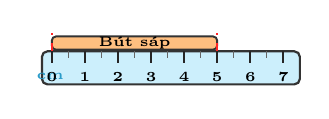
\begin{tikzpicture}[scale=0.6]
  \VeThuocChiaCm[cyan]{7}{0,0}
  \VeVatTrenThuoc{0}{5}{orange}{0,0}{Bút sáp}
\end{tikzpicture}
\end{center}
Xét tính đúng hoặc sai của các nhận xét về cách đo:
\choiceTF
{\True Đặt điểm đầu của vật trùng với vạch số $0$ của thước.}
{\True Đặt mép thước thẳng dọc theo chiều dài của vật cần đo.}
{Điểm cuối của vật trùng với vạch nào thì vật dài bằng vạch đó trừ đi $1\text{ cm}$.}
{\True Điểm cuối của vật trùng với vạch số $5$, vậy chiếc bút dài đúng $5\text{ cm}$.}
\loigiai{
\begin{itemize}
  \item a) \textbf{Đúng}: Luôn đặt một đầu vật ngay vạch $0$.
  \item b) \textbf{Đúng}: Mép thước áp sát vật.
  \item c) \textbf{Sai}: Điểm cuối trùng vạch nào thì vật dài đúng bằng số đó.
  \item d) \textbf{Đúng}: Vật dài $5\text{ cm}$.
\end{itemize}
}
\end{ex}

% CÂU 16: So sánh các độ dài
\begin{ex} %[1H7V26]
Các tấm thẻ ghi số đo độ dài:
\begin{center}
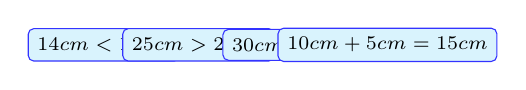
\begin{tikzpicture}[scale=0.6]
  \node[draw=blue!80, fill=cyan!15, rounded corners=2pt, font=\bfseries\scriptsize] at (-3,0) {$14\text{ cm} < 17\text{ cm}$};
  \node[draw=blue!80, fill=cyan!15, rounded corners=2pt, font=\bfseries\scriptsize] at (-1,0) {$25\text{ cm} > 20\text{ cm}$};
  \node[draw=blue!80, fill=cyan!15, rounded corners=2pt, font=\bfseries\scriptsize] at (1,0) {$30\text{ cm} = 3\text{ cm}$};
  \node[draw=blue!80, fill=cyan!15, rounded corners=2pt, font=\bfseries\scriptsize] at (3,0) {$10\text{ cm} + 5\text{ cm} = 15\text{ cm}$};
\end{tikzpicture}
\end{center}
Xét tính đúng hoặc sai của các phép so sánh sau:
\choiceTF
{\True Phép so sánh $14\text{ cm} < 17\text{ cm}$ là đúng.}
{\True Phép so sánh $25\text{ cm} > 20\text{ cm}$ là đúng.}
{Phép so sánh $30\text{ cm} = 3\text{ cm}$ là đúng.}
{\True Phép so sánh $10\text{ cm} + 5\text{ cm} = 15\text{ cm}$ là đúng.}
\loigiai{
\begin{itemize}
  \item a) \textbf{Đúng}: $14 < 17$.
  \item b) \textbf{Đúng}: $25 > 20$.
  \item c) \textbf{Sai}: $30\text{ cm} > 3\text{ cm}$ (không thể bằng nhau).
  \item d) \textbf{Đúng}: $10 + 5 = 15\text{ cm}$.
\end{itemize}
}
\end{ex}

\newpage
% --- TRANG 5: CÂU 17 ĐẾN CÂU 20 (TRẢ LỜI NGẮN / ĐIỀN SỐ) ---

\textbf{Phần 3. Trả lời ngắn}
\setcounterpageref{ex}{0}

% CÂU 17: Phép tính cộng xăng-ti-mét
\begin{ex} %[1H7H26]
Tính tổng độ dài hai đoạn thẳng trên thước kẻ:
\begin{center}

\begin{tikzpicture}[scale=0.65]
  \draw[fill=yellow!30, draw=blue!80, line width=0.7pt, rounded corners=2pt] (-2.2,-0.4) rectangle (2.2,0.4);
  \node[font=\bfseries\normalsize, color=blue!90!black] at (0,0) {$7\text{ cm} + 8\text{ cm} = \dots\text{ cm}$};
\end{tikzpicture}
\end{center}
Kết quả của phép tính trên là bao nhiêu xăng-ti-mét?
\textit{Trả lời:} \raisebox{-2pt}{\tcbox[colframe=blue!80!black,colback=white,size=small,arc=3pt]{$15$}}
\loigiai{
$7 + 8 = 15\text{ cm}$.\\
\textbf{Đáp số: $15$.}
}
\end{ex}

% CÂU 18: Phép tính trừ xăng-ti-mét
\begin{ex} %[1H7H26]
Tính hiệu độ dài trên thước kẻ:
\begin{center}

\begin{tikzpicture}[scale=0.65]
  \draw[fill=pink!30, draw=red!80, line width=0.7pt, rounded corners=2pt] (-2.2,-0.4) rectangle (2.2,0.4);
  \node[font=\bfseries\normalsize, color=red!90!black] at (0,0) {$19\text{ cm} - 6\text{ cm} = \dots\text{ cm}$};
\end{tikzpicture}
\end{center}
Kết quả của phép tính trên là bao nhiêu xăng-ti-mét?
\textit{Trả lời:} \raisebox{-2pt}{\tcbox[colframe=blue!80!black,colback=white,size=small,arc=3pt]{$13$}}
\loigiai{
$19 - 6 = 13\text{ cm}$.\\
\textbf{Đáp số: $13$.}
}
\end{ex}

% CÂU 19: Bài toán cắt bớt sợi dây
\begin{ex} %[1H7V26]
Sợi dây ban đầu dài $25\text{ cm}$, sau đó cắt đi một đoạn $10\text{ cm}$:
\begin{center}
\begin{tikzpicture}[scale=0.65]
  \draw[line width=2pt, green!70!black] (0,0) -- (3.0,0) node[midway, above, font=\bfseries\tiny] {Còn lại ? cm};
  \draw[line width=2pt, gray!60, dashed] (3.0,0) -- (5.0,0) node[midway, above, font=\bfseries\tiny] {Cắt $10\text{ cm}$};
  \draw[line width=0.8pt, stealth-stealth, blue!85] (0,-0.35) -- (5.0,-0.35) node[midway, below, font=\bfseries\tiny] {Cả đoạn dây: $25\text{ cm}$};
\end{tikzpicture}
\end{center}
Hỏi đoạn dây còn lại dài bao nhiêu xăng-ti-mét?
\textit{Trả lời:} \raisebox{-2pt}{\tcbox[colframe=blue!80!black,colback=white,size=small,arc=3pt]{$15$}}
\loigiai{
Đoạn dây còn lại dài là: $25 - 10 = 15\text{ cm}$.\\
\textbf{Đáp số: $15$.}
}
\end{ex}

% CÂU 20: Vận dụng cao - Tính giá trị biểu thức
\begin{ex} %[1H7C26]
Tìm số thích hợp điền vào dấu \textbf{?} trong ô mật mã:
\begin{center}

\begin{tikzpicture}[scale=0.65]
  \draw[fill=yellow!70!orange, draw=black, line width=0.8pt, rounded corners=3pt] (-3.2,-0.45) rectangle (3.2,0.45);
  \node[font=\bfseries\normalsize, color=blue!95!black] at (0,0) {
    $40\text{ cm} + 20\text{ cm} - 30\text{ cm} = \text{\textbf{?}}\text{ cm}$
  };
\end{tikzpicture}
\end{center}
Số thích hợp để thay thế dấu \textbf{?} là bao nhiêu?
\textit{Trả lời:} \raisebox{-2pt}{\tcbox[colframe=blue!80!black,colback=white,size=small,arc=3pt]{$30$}}
\loigiai{
Thực hiện lần lượt từ trái sang phải:\\
$40 + 20 = 60\text{ cm}$; sau đó $60 - 30 = 30\text{ cm}$.\\
\textbf{Đáp số: $30$.}
}
\end{ex}
